\section{Imperfect surfaces of the plate and the sphere}
\label{sec:3:imperfect-plates}

In practice, the surfaces of the sphere and plate are not perfectly flat and contain imperfections, leading to small, localized variations in the sphere-plate separation and consequently to slight changes in the Casimir energy. 
While in reality, both the sphere and the plate have rough surfaces, we limit ourselves to the case where the plate is rough and the sphere is smooth, as we do not expect any fundamental changes.
Under the PFA, the Casimir interaction solely depends on the surface-to-surface separation $\mathscr{L}$ and thus, all irregularities on the sphere's surface can effectively be modeled as an equivalent roughness on the plate.
To quantify and estimate the impact of uneven surfaces on the Casimir energy, several representative types of plate imperfections with characteristic amplitude $\Delta \mathscr{L}$ shown in \cref{fig:3:imperfect-plates} have been studied with numerical methods.
\begin{figure}[!htbp]
  \centering
  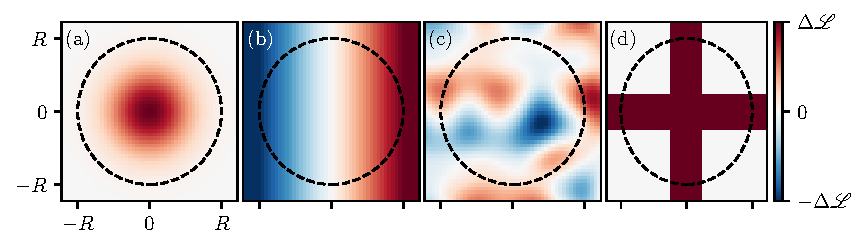
\includegraphics[width=\textwidth]{../figures/casimir/imperfect-plates-advanced-colorbar.pdf}
  \caption{A selection of imperfect plates. \textbf{(a)} A simple gaussian deformation in the same size as the sphere. \textbf{(b)} Linearly inclining plate or a tilted flat plate. \textbf{(c)} Uneven and noisy but uniformly random surface realized using \textit{Perlin noise} \cite{Perlin_1985}. \textbf{(d)} A cross-shape in the center of the plate.}
  \label{fig:3:imperfect-plates}
\end{figure}
\begin{enumerate}
  \item[\textbf{(a)}] A \textit{gaussian shaped bump or dip} in the plate can be used to describe a range of possible local deformations comparable in size to the sphere. 
  For a small shield ($r_s \approx R$), thermal vibrations resemble these deformations, as discussed in \cref{cha:the-shield}.
  Displacements with positive or negative amplitudes $\pm \Delta \mathscr{L}$ following a Gaussian profile were studied.

  \item[\textbf{(b)}] If the characteristic length scale of imperfections is much larger than the sphere's radius and the sphere is sufficiently close to the plate, it experiences a nearly linear gradient in the plate's surface height, effectively behaving as though the plate was tilted. These \textit{linear deflection} can describe thermal vibrations for larger shields $r_s \ll R$. At small gradients, variations in the Casimir potential cancel out in first order since the potential in the PFA $1/(\mathscr{L} \pm \Delta \mathscr{L})^2 \sim 1/\mathscr{L}^2 \mp 2\Delta \mathscr{L}/\mathscr{L}^3$ depends linearly on the deflection. As a result, no significant change in the total attraction force is expected.
  
  \item[\textbf{(c)}] Similarly negligible are \textit{random noisy but uniformly distributed deformations}, provided the typical length scale of the noise is smaller than the sphere's radius. Here, the noise was modeled using \textit{Perlin noise} \cite{Perlin_1985}, which produces smooth pseudo-random surface textures commonly used in computer science to imitate surface roughness. Equidistant grid-points are defined, each of which is assigned with a pseudo-random gradient. The noise function follows this gradient in the vicinity of a grid-point and the interpolation between points generates smooth transitions. Due to the uniformness, no large deviations from an ideal flat plate are expected.
  
  \item[\textbf{(d)}] Structural features on the plate, such as a \textit{centered cross}, may enhance the stability and rigidity of the shield, potentially reducing thermal vibrations. However, the effects of such features, including amplification of the Casimir interaction, must be investigated further.
\end{enumerate}
The resulting Casimir potentials between a macroscopic sphere and the imperfect surfaces were numerically calculated in the PFA and are shown in \cref{fig:3:casimir-imperfect-plates}.
\begin{figure}[!htbp]
  \centering
  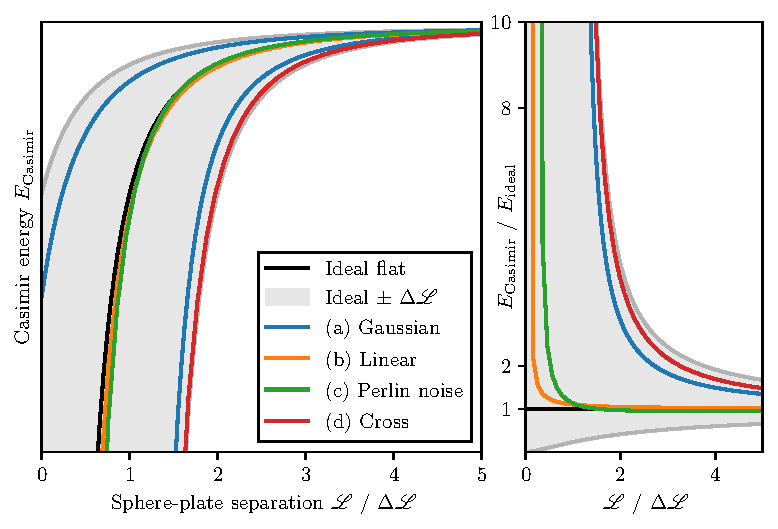
\includegraphics[width=\textwidth]{../figures/casimir/casimir-potential-imperfect-plates-relative.pdf}
  \caption{Casimir energy between a sphere and plates with surface imperfections shown in \cref{fig:3:imperfect-plates}. 
  The gaussian deformation (blue) was calculated for displacements with amplitude $\pm\Delta\mathscr{L}$. The shaded region bounds all imperfections and represents the Casimir energy between a flat plate moved $\pm\Delta\mathscr{L}$ closer or farther to the sphere. In the limit $\Delta \mathscr{L} \ll \mathscr{L}$, all imperfections are negligible.}
  \label{fig:3:casimir-imperfect-plates}
\end{figure}
All imperfections are bounded by the potential between a sphere and a perfectly flat ideal plate moved by a distance $\Delta \mathscr{L}$ closer or farther.
This is symbolized by the gray region in \cref{fig:3:casimir-imperfect-plates}.
For the gaussian distributions, this overestimation is not particularly large and especially for large structures, like the cross, this bound is practically reached.
As expected, the uniformly distributed noise as well as a slightly tilted plane do not increase the Casimir potential substantially even at small separations.
For small imperfections or large separations, plate imperfections are negligible as the relative effect decreases with $\Delta \mathscr{L}/\mathscr{L} \rightarrow 0$.
However, the considerations made in this section are particularly important for small shields the size of the particles and close distances.